
%% bare_jrnl.tex
%% V1.3
%% 2007/01/11
%% by Michael Shell
%% see http://www.michaelshell.org/
%% for current contact information.
%%
%% This is a skeleton file demonstrating the use of IEEEtran.cls
%% (requires IEEEtran.cls version 1.7 or later) with an IEEE journal paper.
%%
%% Support sites:
%% http://www.michaelshell.org/tex/ieeetran/
%% http://www.ctan.org/tex-archive/macros/latex/contrib/IEEEtran/
%% and
%% http://www.ieee.org/



% *** Authors should verify (and, if needed, correct) their LaTeX system  ***
% *** with the testflow diagnostic prior to trusting their LaTeX platform ***
% *** with production work. IEEE's font choices can trigger bugs that do  ***
% *** not appear when using other class files.                            ***
% The testflow support page is at:
% http://www.michaelshell.org/tex/testflow/


%%*************************************************************************
%% Legal Notice:
%% This code is offered as-is without any warranty either expressed or
%% implied; without even the implied warranty of MERCHANTABILITY or
%% FITNESS FOR A PARTICULAR PURPOSE! 
%% User assumes all risk.
%% In no event shall IEEE or any contributor to this code be liable for
%% any damages or losses, including, but not limited to, incidental,
%% consequential, or any other damages, resulting from the use or misuse
%% of any information contained here.
%%
%% All comments are the opinions of their respective authors and are not
%% necessarily endorsed by the IEEE.
%%
%% This work is distributed under the LaTeX Project Public License (LPPL)
%% ( http://www.latex-project.org/ ) version 1.3, and may be freely used,
%% distributed and modified. A copy of the LPPL, version 1.3, is included
%% in the base LaTeX documentation of all distributions of LaTeX released
%% 2003/12/01 or later.
%% Retain all contribution notices and credits.
%% ** Modified files should be clearly indicated as such, including  **
%% ** renaming them and changing author support contact information. **
%%
%% File list of work: IEEEtran.cls, IEEEtran_HOWTO.pdf, bare_adv.tex,
%%                    bare_conf.tex, bare_jrnl.tex, bare_jrnl_compsoc.tex
%%*************************************************************************

% Note that the a4paper option is mainly intended so that authors in
% countries using A4 can easily print to A4 and see how their papers will
% look in print - the typesetting of the document will not typically be
% affected with changes in paper size (but the bottom and side margins will).
% Use the testflow package mentioned above to verify correct handling of
% both paper sizes by the user's LaTeX system.
%
% Also note that the "draftcls" or "draftclsnofoot", not "draft", option
% should be used if it is desired that the figures are to be displayed in
% draft mode.
%
\documentclass[journal]{IEEEtran}
%
% If IEEEtran.cls has not been installed into the LaTeX system files,
% manually specify the path to it like:
% \documentclass[journal]{../sty/IEEEtran}





% Some very useful LaTeX packages include:
% (uncomment the ones you want to load)


% *** MISC UTILITY PACKAGES ***
%
%\usepackage{ifpdf}
% Heiko Oberdiek's ifpdf.sty is very useful if you need conditional
% compilation based on whether the output is pdf or dvi.
% usage:
% \ifpdf
%   % pdf code
% \else
%   % dvi code
% \fi
% The latest version of ifpdf.sty can be obtained from:
% http://www.ctan.org/tex-archive/macros/latex/contrib/oberdiek/
% Also, note that IEEEtran.cls V1.7 and later provides a builtin
% \ifCLASSINFOpdf conditional that works the same way.
% When switching from latex to pdflatex and vice-versa, the compiler may
% have to be run twice to clear warning/error messages.






% *** CITATION PACKAGES ***
%
\usepackage{cite}
% cite.sty was written by Donald Arseneau
% V1.6 and later of IEEEtran pre-defines the format of the cite.sty package
% \cite{} output to follow that of IEEE. Loading the cite package will
% result in citation numbers being automatically sorted and properly
% "compressed/ranged". e.g., [1], [9], [2], [7], [5], [6] without using
% cite.sty will become [1], [2], [5]--[7], [9] using cite.sty. cite.sty's
% \cite will automatically add leading space, if needed. Use cite.sty's
% noadjust option (cite.sty V3.8 and later) if you want to turn this off.
% cite.sty is already installed on most LaTeX systems. Be sure and use
% version 4.0 (2003-05-27) and later if using hyperref.sty. cite.sty does
% not currently provide for hyperlinked citations.
% The latest version can be obtained at:
% http://www.ctan.org/tex-archive/macros/latex/contrib/cite/
% The documentation is contained in the cite.sty file itself.






% *** GRAPHICS RELATED PACKAGES ***
%
\ifCLASSINFOpdf
  \usepackage[pdftex]{graphicx}
  % declare the path(s) where your graphic files are
  % \graphicspath{{../pdf/}{../jpeg/}}
  % and their extensions so you won't have to specify these with
  % every instance of \includegraphics
  % \DeclareGraphicsExtensions{.pdf,.jpeg,.png}
\else
  % or other class option (dvipsone, dvipdf, if not using dvips). graphicx
  % will default to the driver specified in the system graphics.cfg if no
  % driver is specified.
  % \usepackage[dvips]{graphicx}
  % declare the path(s) where your graphic files are
  % \graphicspath{{../eps/}}
  % and their extensions so you won't have to specify these with
  % every instance of \includegraphics
  % \DeclareGraphicsExtensions{.eps}
\fi
% graphicx was written by David Carlisle and Sebastian Rahtz. It is
% required if you want graphics, photos, etc. graphicx.sty is already
% installed on most LaTeX systems. The latest version and documentation can
% be obtained at: 
% http://www.ctan.org/tex-archive/macros/latex/required/graphics/
% Another good source of documentation is "Using Imported Graphics in
% LaTeX2e" by Keith Reckdahl which can be found as epslatex.ps or
% epslatex.pdf at: http://www.ctan.org/tex-archive/info/
%
% latex, and pdflatex in dvi mode, support graphics in encapsulated
% postscript (.eps) format. pdflatex in pdf mode supports graphics
% in .pdf, .jpeg, .png and .mps (metapost) formats. Users should ensure
% that all non-photo figures use a vector format (.eps, .pdf, .mps) and
% not a bitmapped formats (.jpeg, .png). IEEE frowns on bitmapped formats
% which can result in "jaggedy"/blurry rendering of lines and letters as
% well as large increases in file sizes.
%
% You can find documentation about the pdfTeX application at:
% http://www.tug.org/applications/pdftex





% *** MATH PACKAGES ***
%
%\usepackage[cmex10]{amsmath}
% A popular package from the American Mathematical Society that provides
% many useful and powerful commands for dealing with mathematics. If using
% it, be sure to load this package with the cmex10 option to ensure that
% only type 1 fonts will utilized at all point sizes. Without this option,
% it is possible that some math symbols, particularly those within
% footnotes, will be rendered in bitmap form which will result in a
% document that can not be IEEE Xplore compliant!
%
% Also, note that the amsmath package sets \interdisplaylinepenalty to 10000
% thus preventing page breaks from occurring within multiline equations. Use:
%\interdisplaylinepenalty=2500
% after loading amsmath to restore such page breaks as IEEEtran.cls normally
% does. amsmath.sty is already installed on most LaTeX systems. The latest
% version and documentation can be obtained at:
% http://www.ctan.org/tex-archive/macros/latex/required/amslatex/math/





% *** SPECIALIZED LIST PACKAGES ***
%
%\usepackage{algorithmic}
% algorithmic.sty was written by Peter Williams and Rogerio Brito.
% This package provides an algorithmic environment fo describing algorithms.
% You can use the algorithmic environment in-text or within a figure
% environment to provide for a floating algorithm. Do NOT use the algorithm
% floating environment provided by algorithm.sty (by the same authors) or
% algorithm2e.sty (by Christophe Fiorio) as IEEE does not use dedicated
% algorithm float types and packages that provide these will not provide
% correct IEEE style captions. The latest version and documentation of
% algorithmic.sty can be obtained at:
% http://www.ctan.org/tex-archive/macros/latex/contrib/algorithms/
% There is also a support site at:
% http://algorithms.berlios.de/index.html
% Also of interest may be the (relatively newer and more customizable)
% algorithmicx.sty package by Szasz Janos:
% http://www.ctan.org/tex-archive/macros/latex/contrib/algorithmicx/




% *** ALIGNMENT PACKAGES ***
%
%\usepackage{array}
% Frank Mittelbach's and David Carlisle's array.sty patches and improves
% the standard LaTeX2e array and tabular environments to provide better
% appearance and additional user controls. As the default LaTeX2e table
% generation code is lacking to the point of almost being broken with
% respect to the quality of the end results, all users are strongly
% advised to use an enhanced (at the very least that provided by array.sty)
% set of table tools. array.sty is already installed on most systems. The
% latest version and documentation can be obtained at:
% http://www.ctan.org/tex-archive/macros/latex/required/tools/


%\usepackage{mdwmath}
%\usepackage{mdwtab}
% Also highly recommended is Mark Wooding's extremely powerful MDW tools,
% especially mdwmath.sty and mdwtab.sty which are used to format equations
% and tables, respectively. The MDWtools set is already installed on most
% LaTeX systems. The lastest version and documentation is available at:
% http://www.ctan.org/tex-archive/macros/latex/contrib/mdwtools/


% IEEEtran contains the IEEEeqnarray family of commands that can be used to
% generate multiline equations as well as matrices, tables, etc., of high
% quality.


%\usepackage{eqparbox}
% Also of notable interest is Scott Pakin's eqparbox package for creating
% (automatically sized) equal width boxes - aka "natural width parboxes".
% Available at:
% http://www.ctan.org/tex-archive/macros/latex/contrib/eqparbox/





% *** SUBFIGURE PACKAGES ***
%\usepackage[tight,footnotesize]{subfigure}
% subfigure.sty was written by Steven Douglas Cochran. This package makes it
% easy to put subfigures in your figures. e.g., "Figure 1a and 1b". For IEEE
% work, it is a good idea to load it with the tight package option to reduce
% the amount of white space around the subfigures. subfigure.sty is already
% installed on most LaTeX systems. The latest version and documentation can
% be obtained at:
% http://www.ctan.org/tex-archive/obsolete/macros/latex/contrib/subfigure/
% subfigure.sty has been superceeded by subfig.sty.



%\usepackage[caption=false]{caption}
%\usepackage[font=footnotesize]{subfig}
% subfig.sty, also written by Steven Douglas Cochran, is the modern
% replacement for subfigure.sty. However, subfig.sty requires and
% automatically loads Axel Sommerfeldt's caption.sty which will override
% IEEEtran.cls handling of captions and this will result in nonIEEE style
% figure/table captions. To prevent this problem, be sure and preload
% caption.sty with its "caption=false" package option. This is will preserve
% IEEEtran.cls handing of captions. Version 1.3 (2005/06/28) and later 
% (recommended due to many improvements over 1.2) of subfig.sty supports
% the caption=false option directly:
%\usepackage[caption=false,font=footnotesize]{subfig}
%
% The latest version and documentation can be obtained at:
% http://www.ctan.org/tex-archive/macros/latex/contrib/subfig/
% The latest version and documentation of caption.sty can be obtained at:
% http://www.ctan.org/tex-archive/macros/latex/contrib/caption/




% *** FLOAT PACKAGES ***
%
%\usepackage{fixltx2e}
% fixltx2e, the successor to the earlier fix2col.sty, was written by
% Frank Mittelbach and David Carlisle. This package corrects a few problems
% in the LaTeX2e kernel, the most notable of which is that in current
% LaTeX2e releases, the ordering of single and double column floats is not
% guaranteed to be preserved. Thus, an unpatched LaTeX2e can allow a
% single column figure to be placed prior to an earlier double column
% figure. The latest version and documentation can be found at:
% http://www.ctan.org/tex-archive/macros/latex/base/



%\usepackage{stfloats}
% stfloats.sty was written by Sigitas Tolusis. This package gives LaTeX2e
% the ability to do double column floats at the bottom of the page as well
% as the top. (e.g., "\begin{figure*}[!b]" is not normally possible in
% LaTeX2e). It also provides a command:
%\fnbelowfloat
% to enable the placement of footnotes below bottom floats (the standard
% LaTeX2e kernel puts them above bottom floats). This is an invasive package
% which rewrites many portions of the LaTeX2e float routines. It may not work
% with other packages that modify the LaTeX2e float routines. The latest
% version and documentation can be obtained at:
% http://www.ctan.org/tex-archive/macros/latex/contrib/sttools/
% Documentation is contained in the stfloats.sty comments as well as in the
% presfull.pdf file. Do not use the stfloats baselinefloat ability as IEEE
% does not allow \baselineskip to stretch. Authors submitting work to the
% IEEE should note that IEEE rarely uses double column equations and
% that authors should try to avoid such use. Do not be tempted to use the
% cuted.sty or midfloat.sty packages (also by Sigitas Tolusis) as IEEE does
% not format its papers in such 
\usepackage{array}

%\ifCLASSOPTIONcaptionsoff
%  \usepackage[nomarkers]{endfloat}
% \let\MYoriglatexcaption\caption
% \renewcommand{\caption}[2][\relax]{\MYoriglatexcaption[#2]{#2}}
%\fi
% endfloat.sty was written by James Darrell McCauley and Jeff Goldberg.
% This package may be useful when used in conjunction with IEEEtran.cls'
% captionsoff option. Some IEEE journals/societies require that submissions
% have lists of figures/tables at the end of the paper and that
% figures/tables without any captions are placed on a page by themselves at
% the end of the document. If needed, the draftcls IEEEtran class option or
% \CLASSINPUTbaselinestretch interface can be used to increase the line
% spacing as well. Be sure and use the nomarkers option of endfloat to
% prevent endfloat from "marking" where the figures would have been placed
% in the text. The two hack lines of code above are a slight modification of
% that suggested by in the endfloat docs (section 8.3.1) to ensure that
% the full captions always appear in the list of figures/tables - even if
% the user used the short optional argument of \caption[]{}.
% IEEE papers do not typically make use of \caption[]'s optional argument,
% so this should not be an issue. A similar trick can be used to disable
% captions of packages such as subfig.sty that lack options to turn off
% the subcaptions:
% For subfig.sty:
% \let\MYorigsubfloat\subfloat
% \renewcommand{\subfloat}[2][\relax]{\MYorigsubfloat[]{#2}}
% For subfigure.sty:
% \let\MYorigsubfigure\subfigure
% \renewcommand{\subfigure}[2][\relax]{\MYorigsubfigure[]{#2}}
% However, the above trick will not work if both optional arguments of
% the \subfloat/subfig command are used. Furthermore, there needs to be a
% description of each subfigure *somewhere* and endfloat does not add
% subfigure captions to its list of figures. Thus, the best approach is to
% avoid the use of subfigure captions (many IEEE journals avoid them anyway)
% and instead reference/explain all the subfigures within the main caption.
% The latest version of endfloat.sty and its documentation can obtained at:
% http://www.ctan.org/tex-archive/macros/latex/contrib/endfloat/
%
% The IEEEtran \ifCLASSOPTIONcaptionsoff conditional can also be used
% later in the document, say, to conditionally put the References on a 
% page by themselves.

% *** PDF, URL AND HYPERLINK PACKAGES ***
%
\usepackage{url}
% url.sty was written by Donald Arseneau. It provides better support for
% handling and breaking URLs. url.sty is already installed on most LaTeX
% systems. The latest version can be obtained at:
% http://www.ctan.org/tex-archive/macros/latex/contrib/misc/
% Read the url.sty source comments for usage information. Basically,
% \url{my_url_here}.





% *** Do not adjust lengths that control margins, column widths, etc. ***
% *** Do not use packages that alter fonts (such as pslatex).         ***
% There should be no need to do such things with IEEEtran.cls V1.6 and later.
% (Unless specifically asked to do so by the journal or conference you plan
% to submit to, of course. )

\usepackage{enumerate}

% correct bad hyphenation here
\hyphenation{}

\newcommand{\direct}{WI-FI Direct\textsuperscript{\texttrademark}}
\newcommand{\ttt}[1]{\texttt{#1}}

\begin{document}
%
% paper title
% can use linebreaks \\ within to get better formatting as desired
\title{A smart-phone and desktop testbed for Vehicolar Networking experimentation}
%
%
% author names and IEEE memberships
% note positions of commas and nonbreaking spaces ( ~ ) LaTeX will not break
% a structure at a ~ so this keeps an author's name from being broken across
% two lines.
% use \thanks{} to gain access to the first footnote area
% a separate \thanks must be used for each paragraph as LaTeX2e's \thanks
% was not built to handle multiple paragraphs
%

\author{Ambrosin~Moreno,~De~Gaspari~Fabio
%~\IEEEmembership{Computer Science Master Student, Padova University}
        % <-this % stops a space
%\thanks{M. Shell is with the Department of Electrical and Computer Engineering, Georgia Institute of Technology, Atlanta,GA, 30332 USA e-mail: (see http://www.michaelshell.org/contact.html).}% <-this % stops a space
%\thanks{J. Doe and J. Doe are with Anonymous University.}% <-this % stops a space
%\thanks{Manuscript received April 19, 2005; revised January 11, 2007.}
}

% note the % following the last \IEEEmembership and also \thanks - 
% these prevent an unwanted space from occurring between the last author name
% and the end of the author line. i.e., if you had this:
% 
% \author{....lastname \thanks{...} \thanks{...} }
%                     ^------------^------------^----Do not want these spaces!
%
% a space would be appended to the last name and could cause every name on that
% line to be shifted left slightly. This is one of those "LaTeX things". For
% instance, "\textbf{A} \textbf{B}" will typeset as "A B" not "AB". To get
% "AB" then you have to do: "\textbf{A}\textbf{B}"
% \thanks is no different in this regard, so shield the last } of each \thanks
% that ends a line with a % and do not let a space in before the next \thanks.
% Spaces after \IEEEmembership other than the last one are OK (and needed) as
% you are supposed to have spaces between the names. For what it is worth,
% this is a minor point as most people would not even notice if the said evil
% space somehow managed to creep in.



% The paper headers
\markboth{A smart-phone and desktop testbed for Vehicolar Networking experimentation}
{A smart-phone and desktop testbed for Vehicolar Networking experimentation}
% The only time the second header will appear is for the odd numbered pages
% after the title page when using the twoside option.
% 
% *** Note that you probably will NOT want to include the author's ***
% *** name in the headers of peer review papers.                   ***
% You can use \ifCLASSOPTIONpeerreview for conditional compilation here if
% you desire.


% use for special paper notices
%\IEEEspecialpapernotice{(Invited Paper)}

% make the title area
\maketitle


\begin{abstract}
%\boldmath
Generally, testing VANETs protocols can be quite problematic. Real-life simulations are expensive in both economic and temporal terms, so most of the time a software simulation is used. In this document we describe our VANET testbed applications, one for Android and one for Desktops, which can be used to easily test different protocols for vehicolar networks.
To evaluate the performances of our work, we implemented Fast Broadcast algorithm\cite{fastBroadcast}, a Vehicle-to-Vehicle Multi-
Hop Broadcast algorithm used to estimate vehicles' transmission range and to propagate Alert messages through vehicles reducing traversed hops.

\end{abstract}
% IEEEtran.cls defaults to using nonbold math in the Abstract.
% This preserves the distinction between vectors and scalars. However,
% if the journal you are submitting to favors bold math in the abstract,
% then you can use LaTeX's standard command \boldmath at the very start
% of the abstract to achieve this. Many IEEE journals frown on math
% in the abstract anyway.

% Note that keywords are not normally used for peerreview papers.
\begin{IEEEkeywords}
Vehicular Networks, Fast Broadcast, \direct, Android, Raw Socket.
\end{IEEEkeywords}


% For peer review papers, you can put extra information on the cover
% page as needed:
% \ifCLASSOPTIONpeerreview
% \begin{center} \bfseries EDICS Category: 3-BBND \end{center}
% \fi
%
% For peerreview papers, this IEEEtran command inserts a page break and
% creates the second title. It will be ignored for other modes.
\IEEEpeerreviewmaketitle

\section{Introduction}
% The very first letter is a 2 line initial drop letter followed
% by the rest of the first word in caps.
% 
% form to use if the first word consists of a single letter:
% \IEEEPARstart{A}{demo} file is ....
% 
% form to use if you need the single drop letter followed by
% normal text (unknown if ever used by IEEE):
% \IEEEPARstart{A}{}demo file is ....
% 
% Some journals put the first two words in caps:
% \IEEEPARstart{T}{his demo} file is ....
% 
% Here we have the typical use of a "T" for an initial drop letter
% and "HIS" in caps to complete the first word.
\IEEEPARstart{R}{esearch} on Vehicolar Networks makes large use of software simulations, this because it is unfeasible to build a vehicular network of real vehicles that can act as relays of a message that could travel long distances.
To reduce costs, a possible solution is using common and small devices like smartphones to perform real tests carring them on vehicles, or to run simulations taking advantage of the features they offers.
To develop a complete testbed application for mobile devices, different features must be provided:
\begin{itemize}
	\item Possibility to use GPS location or fake positions.
	\item Wireless connectivity.
\end{itemize}
This features are very easy to supply: the most of the smartphones in commerce has GPS and WI-FI devices installed, and their Operating Systems provide APIs to use them.
Our work is exentially composed by two parts:
\begin{itemize}
	\item A distributed Android application, which involves the use of a finite number of devices each running the same application. It lets users to specify fake locations for different devices with random distances between them, in order to simulate an higher number of vehicles, and changes each device's virtual position when needed, or to use real GPS position in case of real tests. Our testbed application uses Android WI-FI technologies for devices communication, expecially \direct standard developed by WI-FI Alliance\textsuperscript{\texttrademark}.
	\item A Java Desktop application for laptops running Fedora. Only fake positions can be used with it, and for what regards connectivity, C Raw Socket where implemented to provide a connection and state free message sending via WI-FI. 
\end{itemize}
Both of our two products have the same architecture, that will be introduced in the next sections. To test our work, we used Fast Broadcast algorithm, which will be briefly introduced in section \ref{sec:fast_broadcast}.


%\section{Related work}


\section{Fast Broadcast Algorithm}
\label{sec:fast_broadcast}
Fast Broadcast Algorithm provides an easy-to-implement method to estimate vehicles' wireless range and to send Alert messages vehicle-to-vehicle covering large distances. The algorithm does not require any pre-existent network infrastructure, and is essentially divided in two phases:
	\begin{itemize}
		\item \emph{Estimation phase}: in this phase time is divided into \textit{turns}, and at each turn $T$ a vehicle (one per turn) sends an \emph{Hello message} containing information about its estimated wireless range and its position. Every vehicle continuously listens for this kind of messages, and uses the information contained in them to update its range estimation.
		\item \emph{Broadcast phase}: 
		once a vehicle receives an \textit{Alert Message}, it must forward it to its neighbors. To prevent network flooding, every vehicle that receives the message computes a \textit{Contention Window}: this window is used to generate a random time to wait before forwarding the message. If the vehicle then receives the same message it was about to forward, it can simply discard it, because someone else already forwarded the message.
	\end{itemize} 
	
This brief introduction, describes roughly the algorithm idea. We will focus on our implementation in the next sections.

\section{Implementation}

We will now briefly describe our implementation main points. In particular we will introduce:
	\begin{enumerate}[A.]
		\item the \textit{technologies} we used;
		\item the \textit{architecture} of our framework;
		\item how devices are \textit{connected};
		\item the mechanism we used to assign and change \textit{virtual positions};
		\item the structure of \textit{exchanged messages}.
	\end{enumerate}
\subsection{Technologies}

Our Android application uses WI-FI connectivity to other devices, especially using \direct standard. Android SDK's APIs from 14 enables the use of this technology to create small wireless networks, where one of the devices is used as an \emph{Access Point}. \direct specification is only available for purchase from WI-FI Alliance\textsuperscript{\texttrademark} website\cite{wifi_direct}.
Basically a network created with Android \direct APIs is called \emph{group}. A \emph{group} has an owner (the access point), and one or more other devices. In the network the only available IP address is group owner's. 
Via APIs provided by the framework, user's permission is required in order to connect to other devices using \direct.

Desktop application ...

\subsection{Architecture}

In figure \ref{fig:architecture} a simple diagram of the architecture used from both Android application and Desktop application is shown. We used a \textit{Event Bus} architectural pattern, in order to obtain a high decoupling degree between all the modules.

\begin{figure}[htbp]
	\centering
	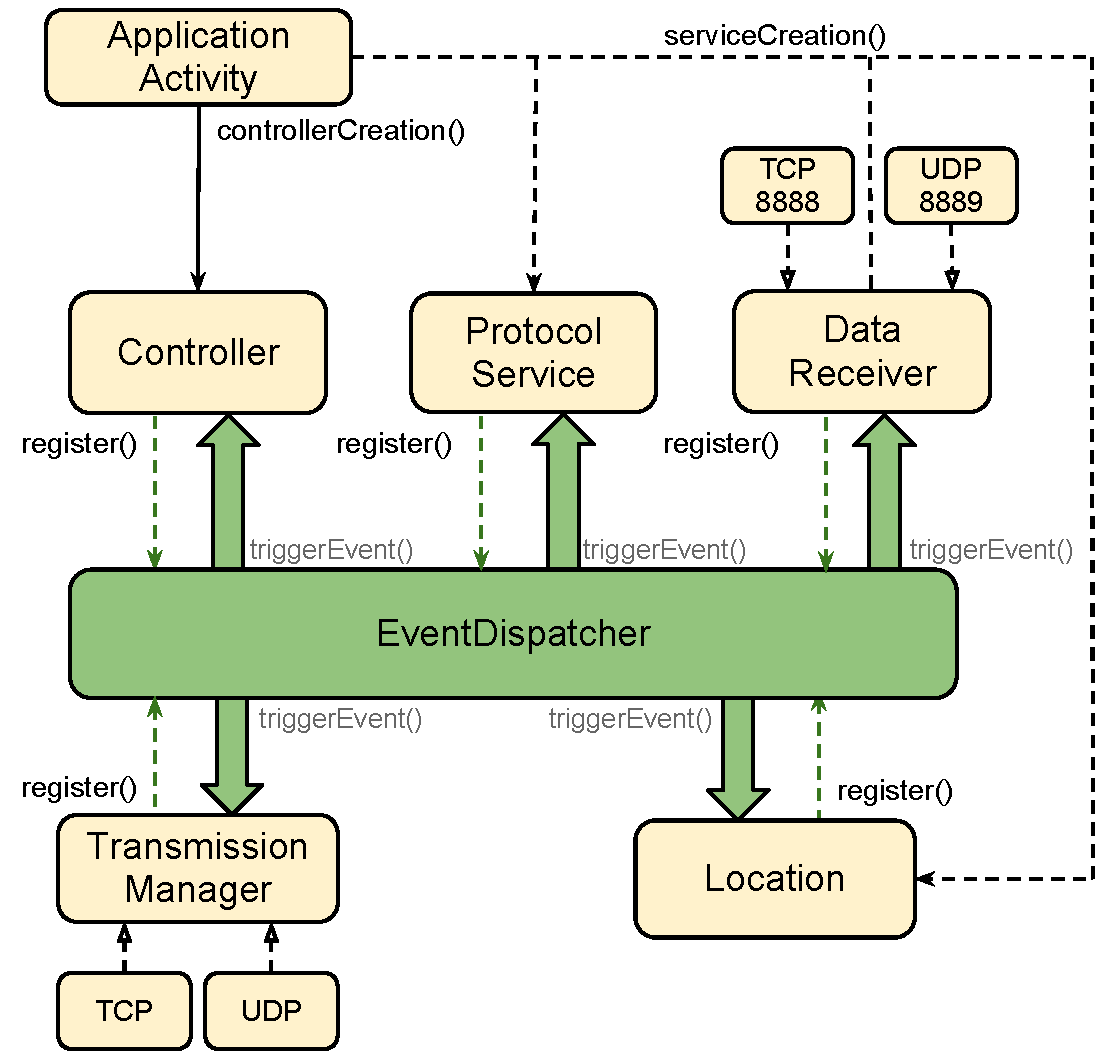
\includegraphics[trim = 10mm 0mm 0mm 0mm,width=3.5in]{imgs/components_architecture.pdf}
	\caption{Graphical representation of application structure.}
	\label{fig:architecture}
\end{figure}

This kind of architecture lets new algorithm modules to be tested, just registering them to the \textit{Event Bus} as \textit{Components}, listening for required events generated by GPS (if exists) and WI-FI, and generating events to exchange data or to move to another position.


\subsection{Devices connection}

Due to the last two \direct features described in the previous section, devices cannot create and destroy connection opportunistically, so for our simulation we had to 
%introduce a connection establishing phase which creates a \direct group and provides to all the devices a complete address map to let them communicate.
manually create a \direct \textit{group} and also to provide devices a complete address map, in order to let them communicate with each
devices.

\begin{figure}[!htbp]
\centering
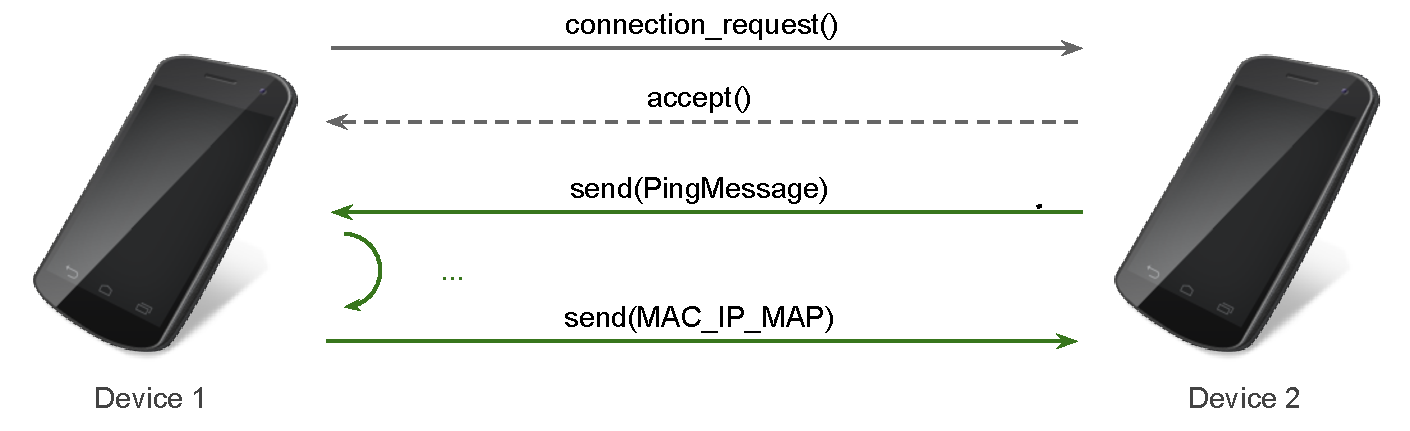
\includegraphics[width=3.6in]{imgs/device_connection_ops.pdf}
\caption{Connection operations sequence}
\label{fig:device_connection}
\end{figure}

Connection setup consists of the following operations:
	\begin{itemize}
		\item One of the devices asks other devices for connection
		\item When a device accepts, it starts a DHCP negotiation with the device which started the connection. If no \direct group exists, a group is created and the device which started the connection becomes the \textit{group owner}. If requesting device is already an owner of a pre-existing group, target device is added to this group. At the end of this phase, each device has an IP address, but only group owner's IP is available via \direct APIs. 
		\item Each device opens a \textit{TCP Server Socket} on port 8888, listening for incoming connections.
		\item When a device connects to a group, it sends a \textit{Ping message} to the \textit{group owner} via a socket. This kind of message is used by the \textit{group owner} to collect MAC and IP addresses of all devices in the group: MAC address is included into the \emph{Ping message} by each device, the second is obtained by the receiver from the incoming Socket information (using Java APIs).
		\item After collecting all the pairs composed by \begin{center}\tt{<MAC address,IP address>}\end{center} from all the devices in the group, \textit{group owner} creates a map, and sends it broadcast, to let devices communicate directly.
	\end{itemize}

Once that all these operations have been done, all the devices are connected and can communicate each other directly via TCP Sockets. An example of a created network is visible in figure \ref{fig:device_network}.

\begin{figure}[!htbp]
\centering
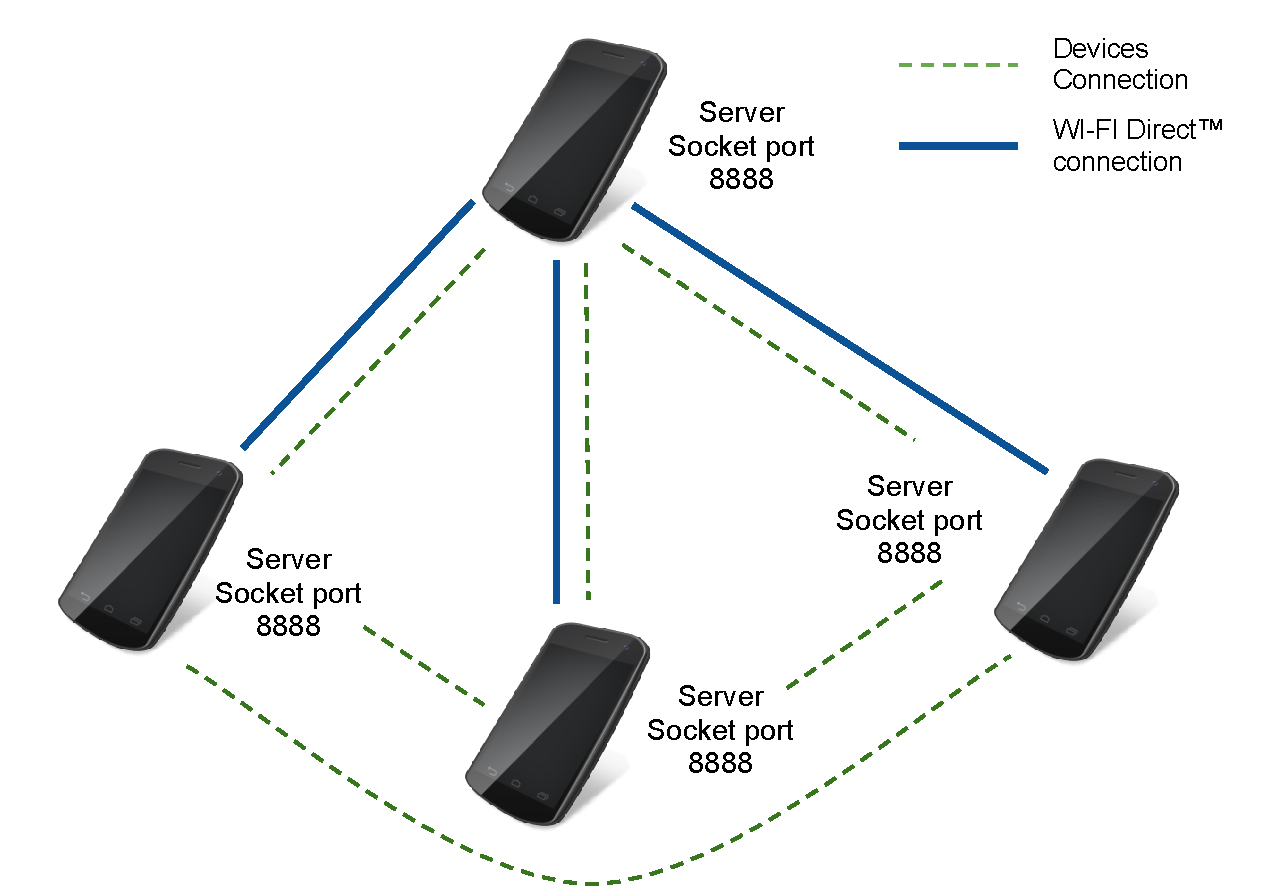
\includegraphics[width=3.6in]{imgs/Devices_network.pdf}
\caption{Network of four devices. Blu lines indicates the \direct group topology, and green lines the logical network}
\label{fig:device_network}
\end{figure}

\subsection{Position changing}
\label{sec:position_change}

To simulate the presence of multiple vehicles a list of fake coordinates can be dinamically assigned to each device during a simulation. Figure \ref{fig:positions} shows an example of how positions are dinamically assigned in the application we built for Android devices in order to implement a testbase application for the Fast Broadcast algorithm (an analogous method is used in Desktop version).

Let's suppose we have four devices, namely A, B, C and D, and suppose we have eight different positions. At the beginning, we have A, B, C and D assigned rispectively to positions 1, 2, 3 and 4. At a certain moment device A broadcasts an \emph{Alert message}. As soon as the messages is sent, device A is assigned to position 5. The other devices compute the \textit{Contention Window} and wait for a random time in the intervall $[0,Contention Window]$ before retransmitting the \emph{Alert}. In figure \ref{fig:positions} devices \textit{Contention Window} is represented as a yellow right triangle, this because it decreases with the increase of the distance from the source. Now let's assume that device C forwards the message because its timeout expires for first: as required by the algorithm, devices B and D will detect the transmission from C and abort the retransmission of A's message. In order to carry on with the simulation, device B (which received C's message from behind) moves from position 2 to position 6, and then reconsider C's message for retransmission. This process continues until the last available position is reached.
In both implementations the starting positions are assigned as soon as the initial setup is completed. In the Android application, the designated \textit{group owner} assigns a progressive number to each device, which represents the line in the position file from which the device should read the first position. Supposing $N$ devices are involved in the simulation, when a device needs to switch position, it will simply skip $N-1$ lines after the current one.
With this iterative mechanism we can distribute a certain number of virtual devices on a route of arbitrary lenght. 
We also use distance filters to simulate real devices range: every time a message is received, the distance from the sender and the receiver is computed and, if it is greater than the (configurable) maximum wireless range, it is discarded.
Position reassignment policy and message filtering based on wireless range, have to be specified in each protocol implementation, and can be achieved generating the corrisponding events.

\begin{figure}[htbp]
\centering
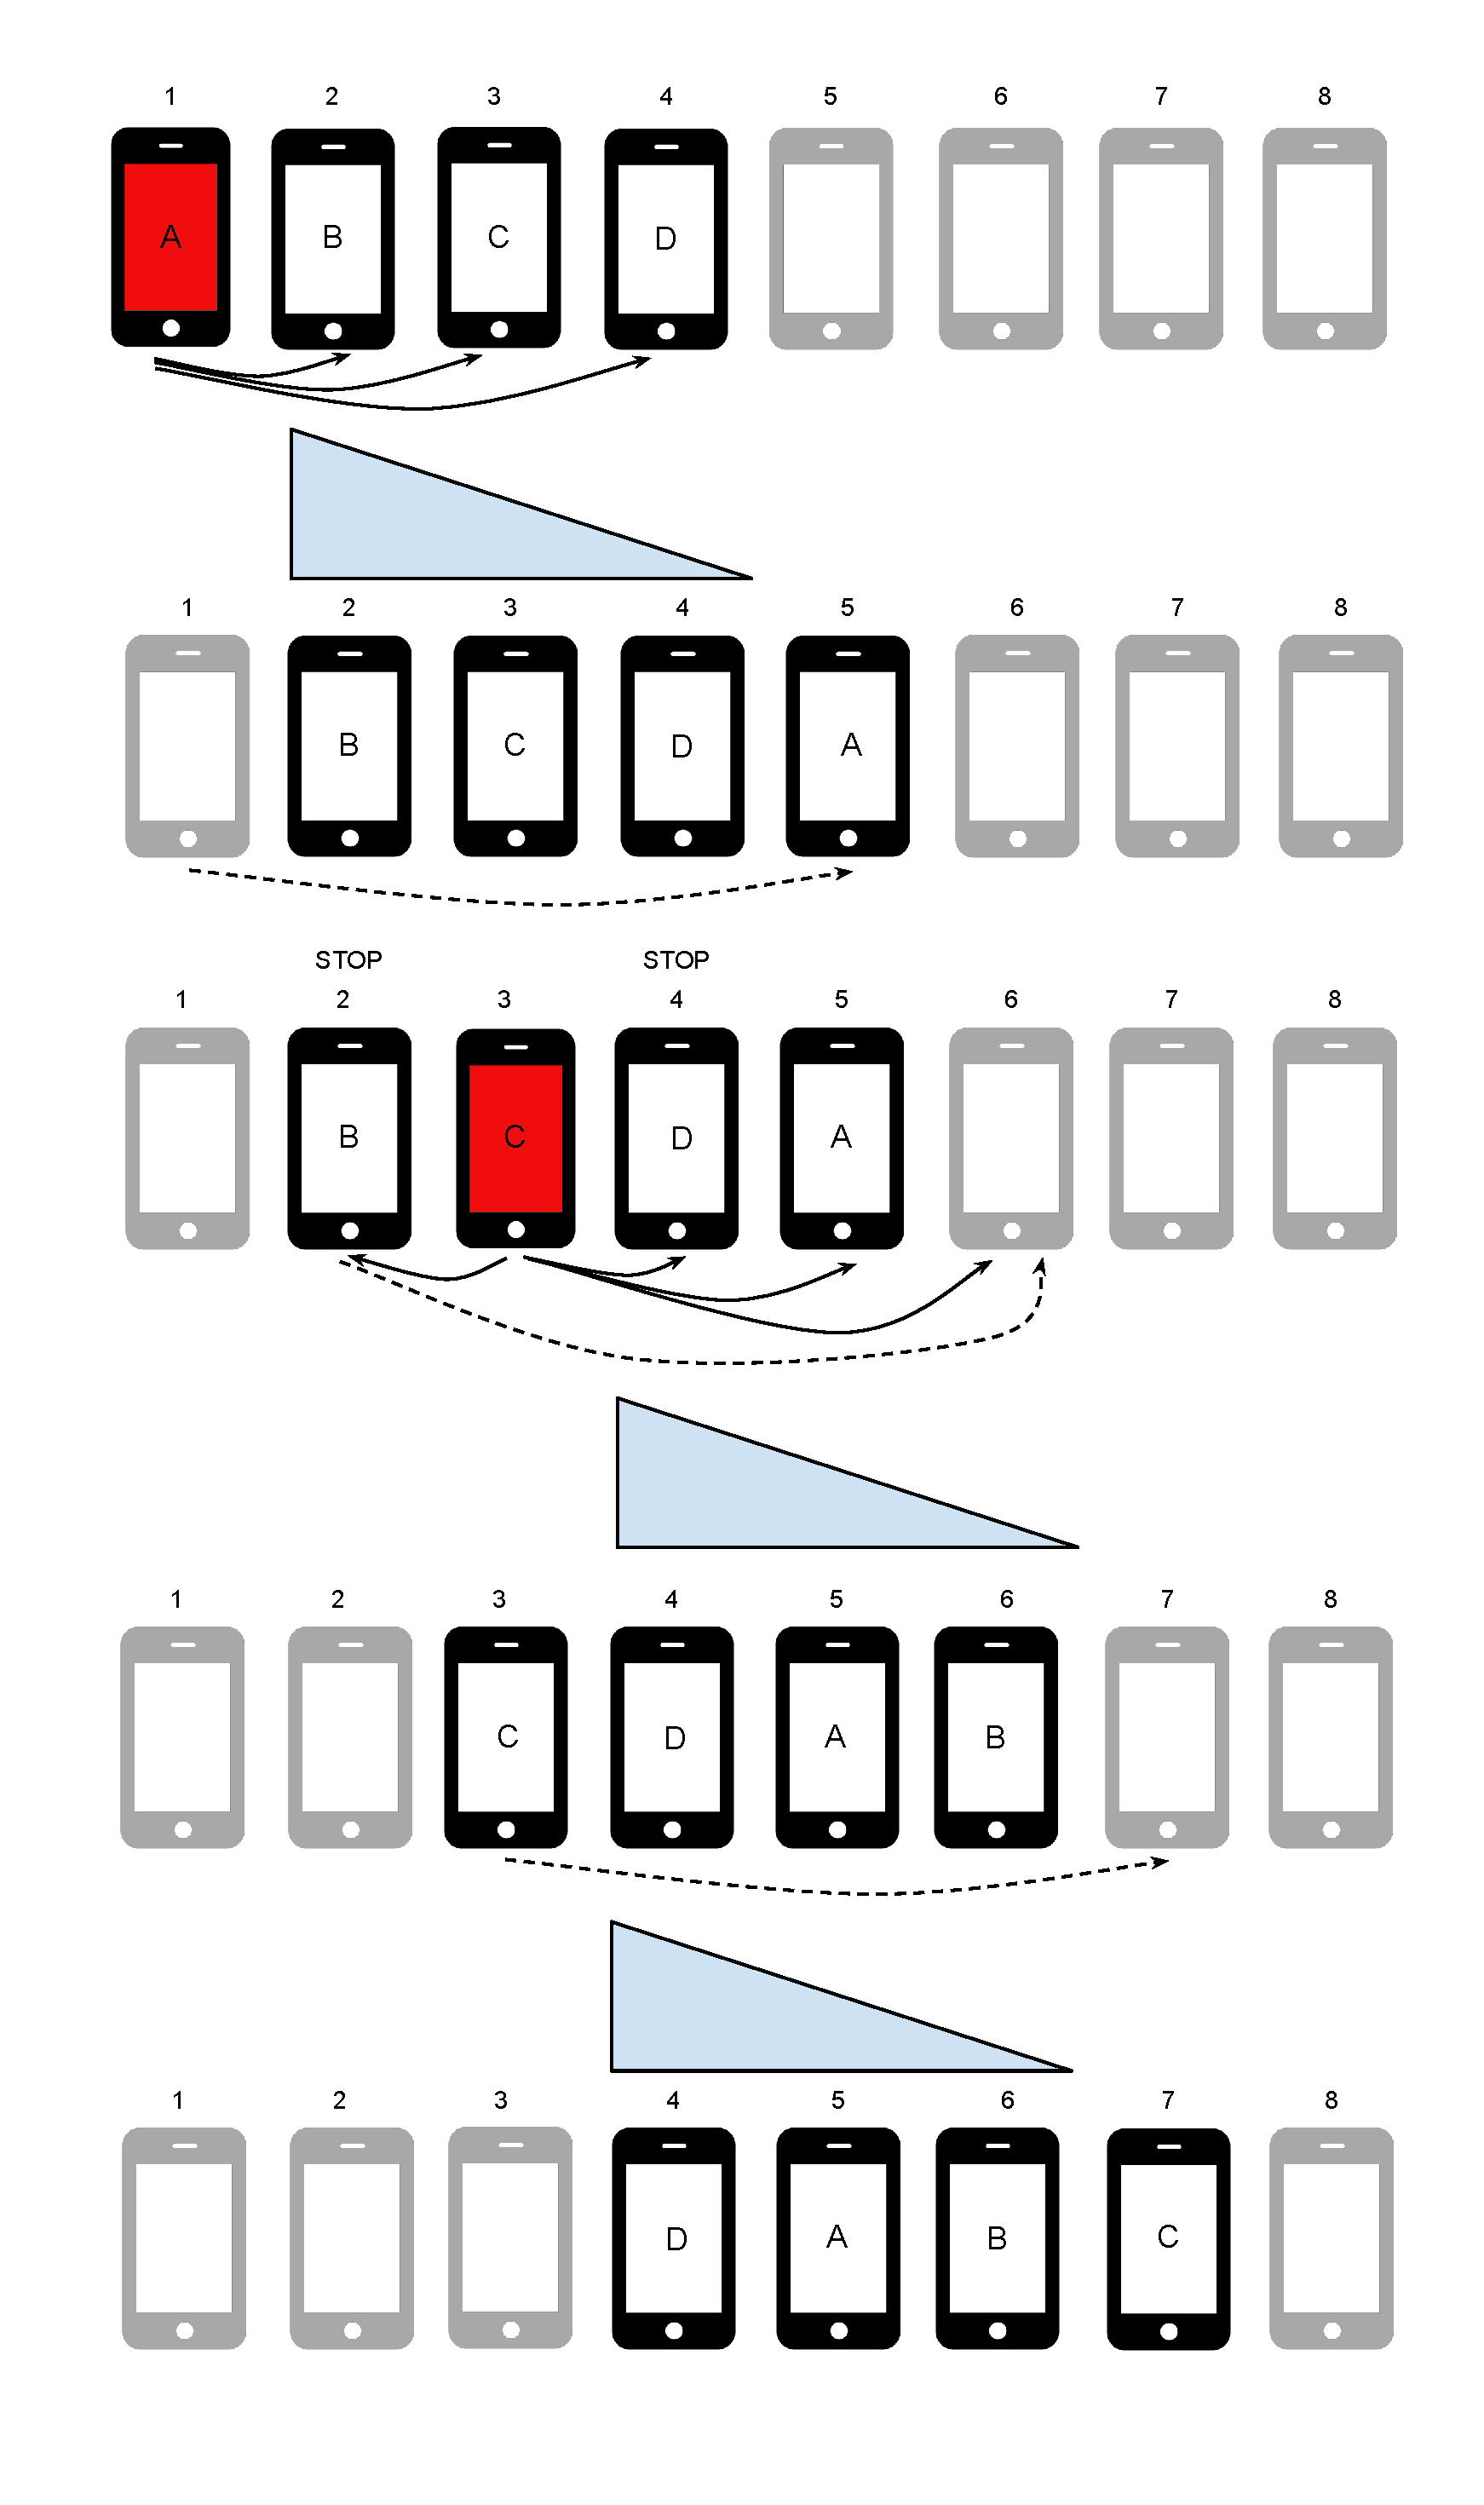
\includegraphics[trim = 10mm 15mm 10mm 10mm ,width=3.5in]{imgs/Positions_1.pdf}
\caption{Devieces positions updating example in Fast Broadcast testbed implementation}
\label{fig:positions}
\end{figure}

\subsection{Exchanged Messages}

Devices send messages encoded as XML strings; the structure of a message is show below in the following listing:
\begin{verbatim}
<message type="..." recipient_id="...">
    <content_block>
        <key>...</key>
        </content>...</content>
    </content_block>
    <content_block>
        <key>...</key>
        </content>...</content>
    </content_block>
    ...
    <content_block>
        <key>...</key>
        </content>...</content>
    </content_block>
</message>
\end{verbatim}
The messages we used contain data espressed as pairs \ttt{<key,content>}. All contained data can be easly converted to Hash Maps objects.

In our implementation, there are four different kinds of messages:
	\begin{description}
		\item[\textbf{Ping message (0)}] \hfill \\
		Application Control Message used to send MAC address to the \textit{group owner}.
		\item[\textbf{Map message (1)}] \hfill \\
		Application Control Message used by the group owner to send the complete \ttt{<MAC address,IP address>} pairs map to all the connected devices.
		\item[\textbf{Alert message (2)}] \hfill \\
		Protocol specific Message used to send an alert to be forwarded to the other connected devices.
		\item[\textbf{Hello message (3)}] \hfill \\
		Fast Broadcast protocol Message corresponding with Fast Broadcast algorithm \textit{Hello message}.
	\end{description}


\section{Experiment}
	\begin{figure}[htbp]
	\centering
	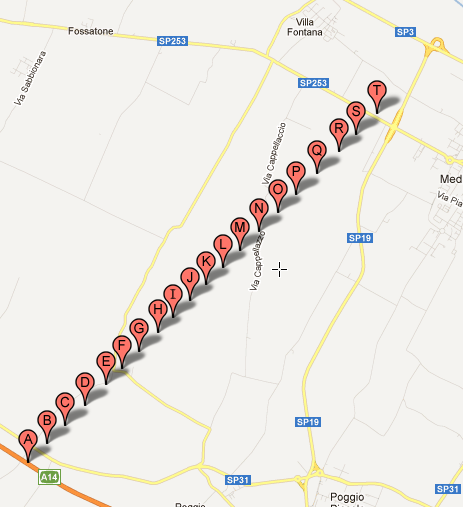
\includegraphics[width=3.4in]{imgs/punti_mappa.png}
	\caption{Fake positions used for the experiment}
	\label{fig:positions_experiment}
	\end{figure}

To test our testbed applications, we implemented Fast Broadcast algorithm (both for Android application and Desktop application). Simulation invelved:
\begin{itemize}
	\item 3 Android devices;
	\item a set of fake position distributed on a straight line, each at a random distance between $275$ and $325$ meters from the following. In figure \ref{fig:positions_experiment} a graphical representation can be seen. They covers approximately $8$ kilometers;
\end{itemize}

We 

\section{Conclusions}
	Our Android application represents a possible implementation, but not the best one. Due to \direct and, more specifically, Android \direct Framework implementation limits, we were forced to heavily modify our architectural design, which resulted in a number of workarounds to simulate a true ad-hoc network communication. We exploited Android \direct framework to create a small network between the various peers and made them communicate via TCP Sockets. This leads to a non scalable simulation, because new devices can only be added at configuration time, and imposes a heavy network load on the peer which acts as a server.
	Moreover, the overhead introduced by the TCP protocol and the execution under the Java Virtual Machine resulted in a difficult validation of the the application results, and added a significant amount of complexity to the coordination of different devices.
	Our first aim was to implement a faster and more dynamic method for data transmission: since in general Vehicolar algorithms do not need a complete network in order to exchange messages (they are basically stateless and connectionless), a viable solution was the use of Data Link level raw sockets to implement a light, connectionless protocol in order to achieve a real ad-hoc network and a behaviour closer to the theoretical. We implemented low level Raw Sockets working on Fedora Operating Systems, but we could not use the developed library on Android devices due to the fact that Android's reduced Linux Kernel lacks of some essential modules. However, we built a desktop application, wich results in higher performances and scalability compared to the Android application. Raw Sockets reduce also connection overhead working at MAC layer level.
	%Unfortunately, after several days of coding and research, we found that in order to obtain all traffic detectable from a device \textit{promiscuous mode} was not sufficient, but an even more battery-comsuming mode was needed, usually referred to as \textit{monitor mode}. Moreover, support for such mode is heavily hardware dependent (not all hardwares support it) and requires direct calls to the network interface device driver, requiring different codes for each device. We concluded that, for the purposes of this project, this was not acceptable in terms of required time and added complexity (considering that, in addition to the forking needed by specific device drivers, the use of unstable and undocumented Android APIs was needed to achieve inter-process communication between the native code, which would be running with root privileges, and the standard Java application).



% You must have at least 2 lines in the paragraph with the drop letter
% (should never be an issue)

% An example of a floating figure using the graphicx package.
% Note that \label must occur AFTER (or within) \caption.
% For figures, \caption should occur after the \includegraphics.
% Note that IEEEtran v1.7 and later has special internal code that
% is designed to preserve the operation of \label within \caption
% even when the captionsoff option is in effect. However, because
% of issues like this, it may be the safest practice to put all your
% \label just after \caption rather than within \caption{}.
%
% Reminder: the "draftcls" or "draftclsnofoot", not "draft", class
% option should be used if it is desired that the figures are to be
% displayed while in draft mode.
%
%\begin{figure}[!t]
%\centering
%\includegraphics[width=2.5in]{myfigure}
% where an .eps filename suffix will be assumed under latex, 
% and a .pdf suffix will be assumed for pdflatex; or what has been declared
% via \DeclareGraphicsExtensions.
%\caption{Simulation Results}
%\label{fig_sim}
%\end{figure}

% Note that IEEE typically puts floats only at the top, even when this
% results in a large percentage of a column being occupied by floats.


% An example of a double column floating figure using two subfigures.
% (The subfig.sty package must be loaded for this to work.)
% The subfigure \label commands are set within each subfloat command, the
% \label for the overall figure must come after \caption.
% \hfil must be used as a separator to get equal spacing.
% The subfigure.sty package works much the same way, except \subfigure is
% used instead of \subfloat.
%
%\begin{figure*}[!t]
%\centerline{\subfloat[Case I]\includegraphics[width=2.5in]{subfigcase1}%
%\label{fig_first_case}}
%\hfil
%\subfloat[Case II]{\includegraphics[width=2.5in]{subfigcase2}%
%\label{fig_second_case}}}
%\caption{Simulation results}
%\label{fig_sim}
%\end{figure*}
%
% Note that often IEEE papers with subfigures do not employ subfigure
% captions (using the optional argument to \subfloat), but instead will
% reference/describe all of them (a), (b), etc., within the main caption.


% An example of a floating table. Note that, for IEEE style tables, the 
% \caption command should come BEFORE the table. Table text will default to
% \footnotesize as IEEE normally uses this smaller font for tables.
% The \label must come after \caption as always.
%
%\begin{table}[!t]
%% increase table row spacing, adjust to taste
%\renewcommand{\arraystretch}{1.3}
% if using array.sty, it might be a good idea to tweak the value of
% \extrarowheight as needed to properly center the text within the cells
%\caption{An Example of a Table}
%\label{table_example}
%\centering
%% Some packages, such as MDW tools, offer better commands for making tables
%% than the plain LaTeX2e tabular which is used here.
%\begin{tabular}{|c||c|}
%\hline
%One & Two\\
%\hline
%Three & Four\\
%\hline
%\end{tabular}
%\end{table}


% Note that IEEE does not put floats in the very first column - or typically
% anywhere on the first page for that matter. Also, in-text middle ("here")
% positioning is not used. Most IEEE journals use top floats exclusively.
% Note that, LaTeX2e, unlike IEEE journals, places footnotes above bottom
% floats. This can be corrected via the \fnbelowfloat command of the
% stfloats package.

% if have a single appendix:
%\appendix[Proof of the Zonklar Equations]
% or
%\appendix  % for no appendix heading
% do not use \section anymore after \appendix, only \section*
% is possibly needed

% use appendices with more than one appendix
% then use \section to start each appendix
% you must declare a \section before using any
% \subsection or using \label (\appendices by itself
% starts a section numbered zero.)
%


%\appendices
%\section{Proof of the First Zonklar Equation}
%Appendix one text goes here.

% you can choose not to have a title for an appendix
% if you want by leaving the argument blank
%\section{}
%Appendix two text goes here.


% use section* for acknowledgement
%\section*{Acknowledgment}



% Can use something like this to put references on a page
% by themselves when using endfloat and the captionsoff option.
\ifCLASSOPTIONcaptionsoff
  \newpage
\fi



% trigger a \newpage just before the given reference
% number - used to balance the columns on the last page
% adjust value as needed - may need to be readjusted if
% the document is modified later
%\IEEEtriggeratref{8}
% The "triggered" command can be changed if desired:
%\IEEEtriggercmd{\enlargethispage{-5in}}

% references section

% can use a bibliography generated by BibTeX as a .bbl file
% BibTeX documentation can be easily obtained at:
% http://www.ctan.org/tex-archive/biblio/bibtex/contrib/doc/
% The IEEEtran BibTeX style support page is at:
% http://www.michaelshell.org/tex/ieeetran/bibtex/
%\bibliographystyle{IEEEtran}
% argument is your BibTeX string definitions and bibliography database(s)
%\bibliography{IEEEabrv,../bib/paper}
%
% <OR> manually copy in the resultant .bbl file
% set second argument of \begin to the number of references
% (used to reserve space for the reference number labels box)
\begin{thebibliography}{1}

\bibitem{fastBroadcast}
%H.~Kopka and P.~W. Daly, \emph{A Guide to \LaTeX}, 3rd~ed.\hskip 1em plus 0.5em minus 0.4em\relax Harlow, England: Addison-Wesley, 1999.
  C.~E.~Palazzi,~S.~Ferretti,~M.~Roccetti,~G.~Pau,~M.~Gerla,~\emph{How Do You Quickly Choreograph Inter-Vehicular Communications? A Fast Vehicle-to-Vehicle Multi-Hop Broadcast Algorithm, Explained},in Proc. of IEEE CCNC 2007, Las Vegas, NV, USA, IEEE Communications Society, Jan 2007.

\bibitem{wifi_direct}
WI-FI Alliance website, 2012, WI-FI Alliance\textsuperscript{\texttrademark}, \url{https://www.wi-fi.org/}

\end{thebibliography}

% biography section
% 
% If you have an EPS/PDF photo (graphicx package needed) extra braces are
% needed around the contents of the optional argument to biography to prevent
% the LaTeX parser from getting confused when it sees the complicated
% \includegraphics command within an optional argument. (You could create
% your own custom macro containing the \includegraphics command to make things
% simpler here.)
%\begin{biography}[{\includegraphics[width=1in,height=1.25in,clip,keepaspectratio]{mshell}}]{Michael Shell}
% or if you just want to reserve a space for a photo:

% You can push biographies down or up by placing
% a \vfill before or after them. The appropriate
% use of \vfill depends on what kind of text is
% on the last page and whether or not the columns
% are being equalized.

%\vfill

% Can be used to pull up biographies so that the bottom of the last one
% is flush with the other column.
%\enlargethispage{-5in}

% that's all folks
\end{document}


